\subsection{Hệ quy chiếu quán tính - phi quán tính}
\begin{frame}{Hệ quy chiếu}
    %Phân biệt giữa các hệ quy chiếu có cùng vận tốc tức thời, nhưng khác về gia tốc (và các đạo hàm bậc cao)
    \begin{center}
        \begin{minipage}[t]{0.45\linewidth}
            \begin{figure}[!htb]
                \centering
                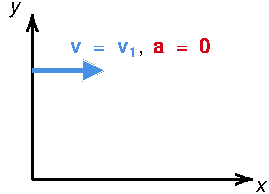
\includegraphics[width=0.9\linewidth]{Figures/FoR_1.pdf}
                \caption{Hệ quy chiếu quán tính}
                \label{fig:FoR_1}
            \end{figure}
        \end{minipage}
        \hspace{5mm}
        \begin{minipage}[t]{0.45\linewidth}            
            \begin{figure}[!htb]
                \centering
                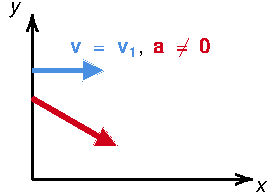
\includegraphics[width=0.9\linewidth]{Figures/FoR_2.pdf}
                \caption{Hệ quy chiếu phi quán tính}
                \label{fig:FoR_2}
            \end{figure}
        \end{minipage}
    \end{center}
\end{frame}

\subsection{Định lý cộng vận tốc và gia tốc}

\begin{frame}{Định lý cộng vận tốc và cộng gia}
    %Chỉ dựa trên công thức

    %Ví dụ: chỉ liên hệ giữa tịnh tiến

    Xét một điểm M trong hệ quy chiếu \(O_1\). Ta sẽ biểu diễn toạ độ, vận tốc, gia tốc của M trong hệ quy chiếu \(O\).

    \begin{center}
        \begin{minipage}{0.4\linewidth}
            \begin{figure}[!htb]
                \centering
                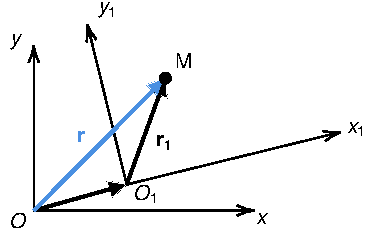
\includegraphics[width=1\linewidth]{Figures/FoR_3.pdf}
                \caption{}
                \label{fig:FoR_3}
            \end{figure}        
        \end{minipage}
        \hspace{1mm}
        \begin{minipage}{0.45\linewidth}
        \begin{equation*}
                \begin{array}{cl}
                \text{Toạ độ} &\left\{
                \begin{array}{cl}
                (O_1): &\mathbf{r_1} \\
                (O): &\mathbf{r} = \mathbf{OO_1} + \mathbf{r_1}
                \end{array}
                \right. 
                \\
                \\
                \text{Vận tốc} &\left\{
                \begin{array}{cl}
                (O_1): &\dot{\mathbf{r}}_1 \\
                (O): &\dot{\mathbf{r}} = \displaystyle \frac{d}{dt}\mathbf{OO}_1 + \dot{\mathbf{r}}_1
                \end{array}
                \right.
                \\
                \\
                \text{Gia tốc} &\left\{
                \begin{array}{cl}
                (O_1): &\ddot{\mathbf{r}}_1 \\
                (O): &\ddot{\mathbf{r}} =\displaystyle \frac{d^2}{dt^2} \mathbf{OO}_1 + \ddot{\mathbf{r}}_1
                \end{array}
                \right.
                \end{array}
        \end{equation*}
        \end{minipage}
    \end{center}
\end{frame}
\begin{frame}{Ví dụ}
    Cho một bánh quay (tâm \(O_1\) cố định), ta đặt hệ quy chiếu ở các điểm \(O,O_1,A,B\). Bánh quay với vận tốc góc \(\omega\), bán kính \(R\).
\begin{center}
    \begin{minipage}{0.5\linewidth}
        \begin{figure}
        \centering
        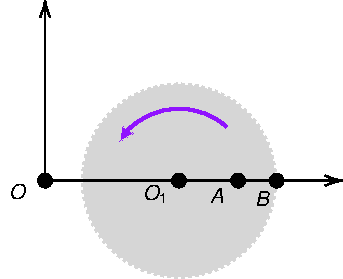
\includegraphics[width=0.8\linewidth]{Figures/FoR_4.pdf}
        \caption{}
        \label{fig:FoR_4}
        \end{figure}        
    \end{minipage}
    \hspace{1mm}
    \begin{minipage}{0.4\linewidth}
        \begin{equation*}
            \begin{array}{ll}
            \mathbf{v_{O_1/B}} &= \mathbf{\omega} \times \mathbf{BO_1} \\ \\
            \mathbf{v_{B/A}} &= \mathbf{\omega} \times \mathbf{BA} \\ \\
            \mathbf{v_{B/O}} &= \mathbf{(-\omega)} \times \mathbf{BO} 
            \end{array}
        \end{equation*}         
    \end{minipage}
\end{center}
\end{frame}


